% Main chapter title
\chapter{Android: Architecture, Permissions, APIs}
\label{ch:related}

% This is for the header on each page
\lhead{Chapter 3. \emph{Android: Architecture, Permissions, APIs}}
\thispagestyle{empty}
Android is widely used operating system for moblie devices. In section 3.1, we will discuss about the architecture of android. In section 3.2, we will discuss permissions required by any application to access the sensitive resources. In Section 3.3, we will give brief idea about APIs.
\section{Architecture}
Android is opensource. Android operating system is based on Linux based-software stack \cite{androidplatformarch}. There are mainly five components in Android software stack. These are:
\begin{enumerate}
    \item Linux Kernel
    \item Native Libraries
    \item Android Runtime
    \item Application Framework
    \item Applications
\end{enumerate}
\begin{figure}[!h]
  \centering
  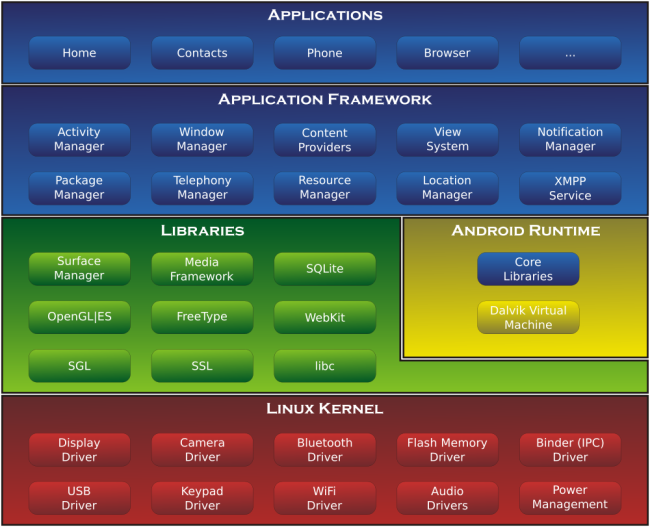
\includegraphics [scale=0.8] {and_arch.png}
  \caption{The Android Software Stack}
  \label{fig:arch}
\end{figure}
\subsection{Linux Kernel}
Linux kernel is root/foundation of the Android platform. Linux kernel is responsible for device drivers, power management, memory management, device management and resource access. Linux kernel includes display driver, camera driver, bluetooth driver, Flash memory driver, Binder (IPC) driver, USB driver, kepad driver, WiFi driver and Audio Driver.

\subsection{Native Libraries}
Native libraries sits on the top of Linux kernel. Some of native libraries are WebKit, OpenGL, FreeType, SQLite, Media, C runtime library (libc), etc. The WebKit is used for browser support, SQLite is used for database, FreeType is used for font support, Media is used for playing and recording audio and video formats.

\subsection{Android Runtime}
Android Runtime contains some core libraries and DVM (Dalvik Virtual Machine) which is responsible to run android application. DVM is similar to JVM but it is more optimized for mobile devices. It comsumes less memory and provides fast performance. ART is written to run multiple virtual machines on low-memory devices. Some of the major features of ART includes the following:
\begin{itemize}
    \item Ahead-of-time (AOT) and just-in-time (JIT) Compilation.
    \item Optimized garbage collection (GC).
    \item Better debugging support, including a dedicated sampling profiler, detailed diagnostic exceptions and crash reporting, and the ability to set watchpoints to monitor specific fields.
\end{itemize}

\subsection{Android Framework}
Android Framework sits on the top of Native libraries and Android runtime. Android framework contains Content provider, View system, Activity manager, Window manager, Telephony manager, resource manager, location manager and XMPP service.

\subsection{Applications}
Last layer of the Android Platform Architecture is applications. It contains applications. All applications such as home, contact, settings, email, dialer, calendar, camera, etc. are using Android framework that uses Native libraries and Android runtime. Android runtime and native libraries are using linear kernel.


%---------------------------------------------------------------------%
%---------------------------------------------------------------------%
\section{Permissions}
If an Android application wants to use any resources such as camera, internet, location, etc., they need permission from the Android operating system to use them. Android marshmallow operating system has more than 200 permissions \cite{androidpermissions}. The main purpose of permission is to protect the user data. Android apps must request permission to access sensitive user data as well as the system features. Depending on the feature, the system might grant the permission automatically or might prompt the user to approve the request. Permissions are divided into several protection level. There are three protection levels that affect third-party apps:
\begin{enumerate}
    \item Normal permissions
    \item Signature permissions
    \item Dangerous permissions
\end{enumerate}
\subsection{Normal Permissions}
Normal permissions are used where an needs to access data or resources outside the app's sandbox but where there is very little risk to the user's privacy or the operation of other apps. According to Android 8.1, following are the list of normal permissions:
\begin{itemize}
    \begin{spacing}{0.9}
    \item \texttt{ACCESS\_LOCATION\_EXTRA\_COMMANDS}
    \item \texttt{ACCESS\_NETWORK\_STATE}
    \item \texttt{ACCESS\_NOTIFICATION\_POLICY}
    \item \texttt{ACCESS\_WIFI\_STATE}
    \item \texttt{BLUETOOTH}
    \item \texttt{BLUETOOTH\_ADMIN}
    \item \texttt{BROADCAST\_STICKY}
    \item \texttt{CHANGE\_NETWORK\_STATE}
    \item \texttt{CHANGE\_WIFI\_MULTICAST\_STATE}
    \item \texttt{CHANGE\_WIFI\_STATE}
    \item \texttt{DISABLE\_KEYGUARD}
    \item \texttt{EXPAND\_STATUS\_BAR}
    \item \texttt{GET\_PACKAGE\_SIZE}
    \item \texttt{INSTALL\_SHORTCUT}
    \item \texttt{INTERNET}
    \item \texttt{KILL\_BACKGROUND\_PROCESSES}
    \item \texttt{MANAGE\_OWN\_CALLS}
    \item \texttt{MODIFY\_AUDIO\_SETTINGS}
    \item \texttt{NFC}
    \item \texttt{READ\_SYNC\_SETTINGS}
    \item \texttt{READ\_SYNC\_STATS}
    \item \texttt{RECEIVE\_BOOT\_COMPLETED}
    \item \texttt{REORDER\_TASKS}
    \item \texttt{REQUEST\_COMPANION\_RUN\_IN\_BACKGROUND}
    \item \texttt{REQUEST\_COMPANION\_USE\_DATA\_IN\_BACKGROUND}
    \item \texttt{REQUEST\_DELETE\_PACKAGES}
    \item \texttt{REQUEST\_IGNORE\_BATTERY\_OPTIMIZATIONS}
    \item \texttt{SET\_ALARM}
    \item \texttt{SET\_WALLPAPER}
    \item \texttt{SET\_WALLPAPER\_HINTS}
    \item \texttt{TRANSMIT\_IR}
    \item \texttt{USE\_FINGERPRINT}
    \item \texttt{VIBRATE}
    \item \texttt{WAKE\_LOCK}
    \item \texttt{WRITE\_SYNC\_SETTINGS}
    \end{spacing}
\end{itemize}
\subsection{Signature Permissions}
The system grants these app permissions at install time, but only when the app that attempts to use a permission is signed by the same certificate as the app that defines the permission. According to Android 8.1, following are the list of signature permissions:
\begin{itemize}
    \begin{spacing}{0.9}
    \item \texttt{BIND\_ACCESSIBILITY\_SERVICE}
    \item \texttt{BIND\_AUTOFILL\_SERVICE}
    \item \texttt{BIND\_CARRIER\_SERVICES}
    \item \texttt{BIND\_CHOOSER\_TARGET\_SERVICE}
    \item \texttt{BIND\_CONDITION\_PROVIDER\_SERVICE}
    \item \texttt{BIND\_DEVICE\_ADMIN}
    \item \texttt{BIND\_DREAM\_SERVICE}
    \item \texttt{BIND\_INCALL\_SERVICE}
    \item \texttt{BIND\_INPUT\_METHOD}
    \item \texttt{BIND\_MIDI\_DEVICE\_SERVICE}
    \item \texttt{BIND\_NFC\_SERVICE}
    \item \texttt{BIND\_NOTIFICATION\_LISTENER\_SERVICE}
    \item \texttt{BIND\_PRINT\_SERVICE}
    \item \texttt{BIND\_SCREENING\_SERVICE}
    \item \texttt{BIND\_TELECOM\_CONNECTION\_SERVICE}
    \item \texttt{BIND\_TEXT\_SERVICE}
    \item \texttt{BIND\_TV\_INPUT}
    \item \texttt{BIND\_VISUAL\_VOICEMAIL\_SERVICE}
    \item \texttt{BIND\_VOICE\_INTERACTION}
    \item \texttt{BIND\_VPN\_SERVICE}
    \item \texttt{BIND\_VR\_LISTENER\_SERVICE}
    \item \texttt{BIND\_WALLPAPER}
    \item \texttt{CLEAR\_APP\_CACHE}
    \item \texttt{MANAGE\_DOCUMENTS}
    \item \texttt{READ\_VOICEMAIL}
    \item \texttt{REQUEST\_INSTALL\_PACKAGES}
    \item \texttt{SYSTEM\_ALERT\_WINDOW}
    \item \texttt{WRITE\_SETTINGS}
    \item \texttt{WRITE\_VOICEMAIL}
    \end{spacing}
\end{itemize}
\subsection{Dangerous Permissions}
Dangerous permissions cover areas where the app wants data or resources that involve the user's private information, or could potentially affect the user's stored data or the operation of other apps. If an app declares that it needs a dangerous permission, the user has to explicitly grant the permission to the app. Until the user approves the permission, your app cannot provide functionality that depends on that permission. According to Android 8.1, following are the list of dangerous permissions:
\begin{itemize}
    \begin{spacing}{0.9}
    \item \texttt{READ\_CALENDAR}
    \item \texttt{WRITE\_CALENDAR}
    \item \texttt{CAMERA}
    \item \texttt{READ\_CONTACTS}
    \item \texttt{WRITE\_CONTACTS}
    \item \texttt{GET\_ACCOUNTS}
    \item \texttt{ACCESS\_FINE\_LOCATION}
    \item \texttt{ACCESS\_COARSE\_LOCATION}
    \item \texttt{RECORD\_AUDIO}
    \item \texttt{READ\_PHONE\_STATE}
    \item \texttt{READ\_PHONE\_NUMBERS}
    \item \texttt{CALL\_PHONE}
    \item \texttt{ANSWER\_PHONE\_CALLS}
    \item \texttt{READ\_CALL\_LOG}
    \item \texttt{WRITE\_CALL\_LOG}
    \item \texttt{ADD\_VOICEMAIL}
    \item \texttt{USE\_SIP}
    \item \texttt{PROCESS\_OUTGOING\_CALLS}
    \item \texttt{BODY\_SENSORS}
    \item \texttt{SEND\_SMS}
    \item \texttt{RECEIVE\_SMS}
    \item \texttt{READ\_SMS}
    \item \texttt{RECEIVE\_WAP\_PUSH}
    \item \texttt{RECEIVE\_MMS}
    \item \texttt{READ\_EXTERNAL\_STORAGE}
    \item \texttt{WRITE\_EXTERNAL\_STORAGE}
    \end{spacing}
\end{itemize}
\section{Application Program Interfaces (APIs)}
The Android API refers to the collection of various software modules which make up the complete Android SDK. If we have to use any functionality of android, then we have to use API corresponding to that functionality.
